\documentclass{ltjbook}
\usepackage{docmute} 
\usepackage{../../myStyle} 

\begin{document}
\chapter{ベイズ推測の基礎2}
前回，ベイズの定理を導入しました。今回はこの定理を，これまで行ってきた推測統計学の枠組みでどのように利用するかを考えていきます。


\section{事前分布と事後分布}
さっそくベイズ法で，実際にパラメータを推定する例を考えてみましょう。

今回は例として，学力テストを取り上げます。
難易度が同じぐらいの10問のテストを受けたとします。推定したいのは回答者の学力です。この能力は，問題に正しく答える比率$\theta$である，と定義します。学力$\theta$は直接観測できず，観測できるのは「正答数」だけです。今回ある回答者が4問正解したとして，学力はどうやって見積もれば良いでしょうか？ というのがここでの課題になります。

ベイズ法による考え方は，基本的にたった2つのステップからなります\footnote{帰無仮説検定より少ない！やったね！}。
\begin{enumerate}
    \item 不確実性，信念の強さを確率によって数量化する(事前分布priorの設定)
    \item 観測データを使って事前の情報/信念を更新し，事後の情報/信念(事後分布posterior)にアップデートする
\end{enumerate}
これだけです。

ではまずステップ1，\keyterm{事前分布}{じぜんぶんぷ}{prior distibution}について考えてみましょう。
\subsection{事前の信念の表し方}
事前分布は，確率のパラメータについて事前に与える分布です。パラメータがどれぐらいになるのか知りたいのに，事前に何かわかっていることがあるっておかしくない？ と思う人もいるかもしれません。
ここで，確率のベイズ的考え方，すなわち確率とは確信の程度を表現しているのだと思って思ってください。不確実で，わからないものを，どの程度わからないのか確率で表現するのです。第\ref{chapter6}講で示したように，推論とは確率の再分配であり，「他に可能性がない」のであれば100\%確からしい，と言えるのでした。逆に「事前にパラメータがどのあたりにあるのかなんて，全くわからない」という場合も，確率で表現することができます。この表現方法として，「どこ」にあるのかわからないのであれば「全部あり得る」と広く広く守備範囲を広げておけば良いことになりますね。確率なので面積は1.0でなければなりませんが，その分うすく伸ばすように考えれば良いのです。

\begin{figure}[ht]
    \centering
    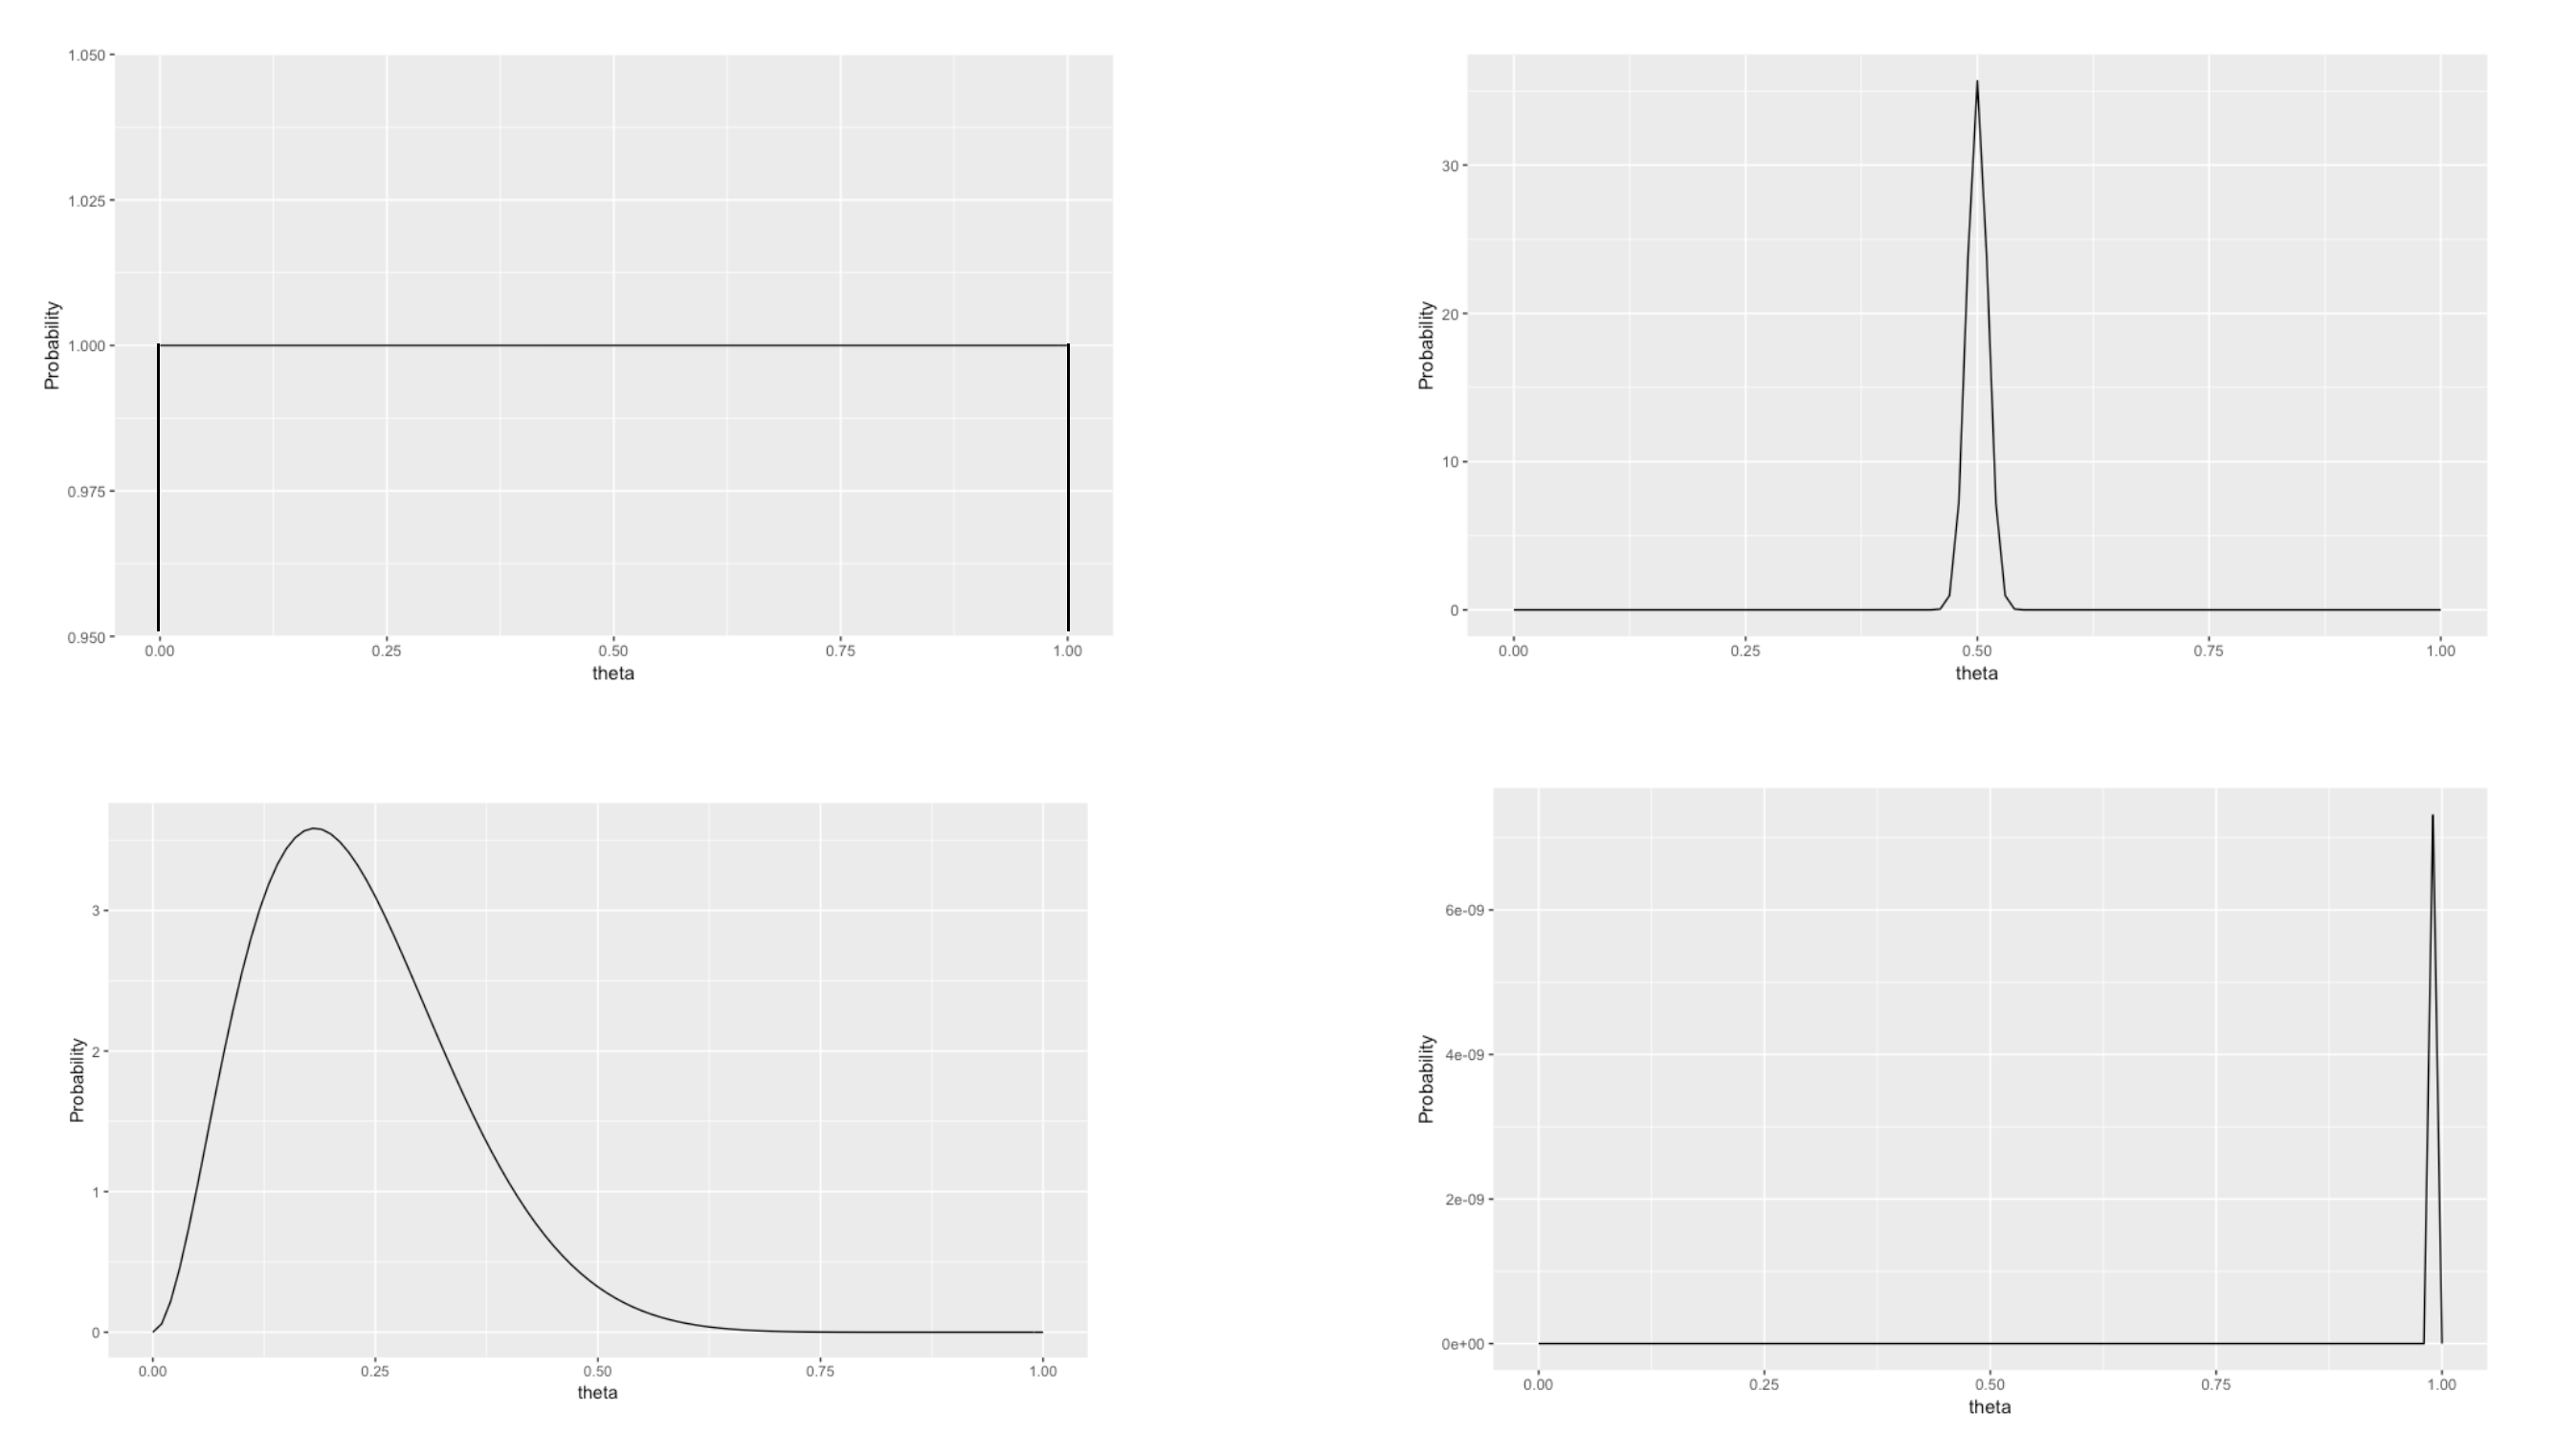
\includegraphics[keepaspectratio,width=12cm]{../images/text25/slide25_01.png}
    \caption{コイントスの出目についての四つの信念}
    \label{fig::25_01}
\end{figure}

図\ref{fig::25_01}に，4つの確率分布を示しました。これらはベルヌーイ分布のパラメータ$\theta$についての，個人の考え方を示していると思ってください。ベルヌーイ分布はコイントスのような，二値の結果を生じさせる試行についての確率分布ですから，確率$\theta$は$0 \le \theta \le 1$の範囲にあるはずです。
図\ref{fig::25_01}の左上は範囲全てにわたってフラットです。つまり，「どこ」にあるとも断言できない，どこにも同じ程度にあるはずだという信念で，言い方を変えると何もはっきりとは言えない，つまりわからない状態を表しています。データを分析するにあたって，事前に何もわからないのであれば，このようにフラットな事前分布(特に\keyterm{一様分布}{いちようぶんぷ}{uniform distribution}といいます)を置けばよく，こういう事前分布の置き方を特に\keyterm{無情報事前分布}{むじょうほうじぜんぶんぷ}{uninformative prior distribution}と呼びます。
図\ref{fig::25_01}の右上は逆に，$\theta=0.5$のあたりにあるはずだ，と思っている人の考え方です。少なくとも0.45，大きくとも0.55ぐらいでしょう，ということなので，かなり確信度の高い(確率分布の幅が狭い)状態にあると言えます。
そこまではっきりわからないけど，でもちょっと裏が出やすそうだなあ，というふんわりと低めの予想をしている人は，図\ref{fig::25_01}の左下のような信念をもっている，と表現できますし，「絶対に表が出る。面しか出ない」と強く信じている人は図\ref{fig::25_01}の右下のようになります。

このように，全くわからないことや，どこかに特定の強い思い入れがあること，あるいはなんとなくこの辺じゃないかと思っていること，など事前の情報を確率分布として表現することは可能なのです。研究の実践場面において，事前に何かわかっていることが「全くない」のであれば，一様分布のような無情報事前分布，あるいはすごく幅の広い弱情報事前分布を置けば良いでしょう。身長や体重などのデータを分析する時に，正規分布を仮定しますが，このような場合は少なくとも負の値をとることはありませんし，いくら背が高い，体重が重いとしても10mや5tになったりするはずはないので，$0\le \mu \le 100000$のような幅で事前分布をおいても構いません。あるいは先行研究などから，ある程度のアタリがつけられるのであれば，その値を中心にふんわりした事前分布を置いたっていいのです。逆にいうと，このように事前分布をおくことで，先行研究との一貫性を持たせたり，先行研究の情報を活用して知見を積み重ねていくことができる，とも言えます\footnote{分散分析や最尤法を考え出したR.A.Fisher先生は，このベイズの考え方がお気に召さなかったようです。研究を始める前になんらかの思い込みを持って取り組むというのはおかしい，データに対してはなんら心構えを持たずに立ち向かうべきだ，という考え方です。Fisher先生のベイズ統計学についての当たりの強さは，\citet{mcgrayne2011theory}などにも記されています。}。

さて今回の例に戻りましょう。この受験生の学力がどれぐらいなのか，事前には全くわかっていません。しかし正答率を考えるのですから，推定値は$0 \le \theta \le 1$の範囲にあるはず。全くわかっていないのですから，この範囲の一様分布を設定しましょう。つまり，特になんの偏見も持たずにデータに立ち向かうという精神を，無情報事前分布で表現するわけです。


\subsection{事後分布の計算}
次にステップ2ですね。アップデートです。アップデートにはベイズの定理を使います。ベイズの定理を改めて見直しておきましょう。次のような式なのでしたね。
\[ P(A|B) = \frac{P(B|A)P(A)}{P(B)}\]
ここで$P()$で表されているのは確率，とだけ言っていましたが，これは離散でも連続でも同じことですので，確率分布と呼びましょう。特に左辺は「結果的にこうなる」という意味ですから，\keyterm{事後分布}{じごぶんぷ}{posterior distribution}と呼ばれます。

この確率的関係(右辺も左辺も全部Pで囲われています！)を，実際に統計的推論の場面で用いることを考えます。左辺にある事後分布は，データをとったうえで，パラメータがどのあたりにあるのかを推論するということを条件付き確率で表しています。つまり，BがデータでAがパラメータ，事後分布$P(A|B)$が「データをとった上でのパラメータの確率」ということです。であれば，右辺にある$P(B|A)$は「パラメータがあった時にデータが出てくる確率」を意味することになります。これってなんでしたっけ？ そう，\keyterm{尤度}{ゆうど}{likelihood}ですね！

さて記号の意味を考えていきますと，$P(A)$はデータを取る前のパラメータの確率，ということになります。これが先ほど説明した\keytermL{事前分布}{じぜんぶんぷ}ですね。

また$P(B)$はデータの確率，ということになります。データの確率？ データが得られるかどうかの確率？ というのはわかるはずがないような気もしますが，前回の乳がんの罹患率の例を思い出すと「あり得るパラメータから考えられる全てのデータが出てくる確率をかき集めたもの」，というようなイメージができるかもしれません。用語としては\keyterm{周辺尤度}{しゅうへんゆうど}{marginal likelihood}といいますが，実践上はこれについて深く考えなくてもよいものであることを後で説明します。のでこれについても話はここまで\footnote{本当の本当は，この周辺尤度というのがデータの適合度などを考える時にとっても重要なものになってくるのですが，心理統計のライトユーザにとっては$t$分布の導出のように「今ここでやらなくてもいい」ものです。興味がある人は\citet{浜田201912}を読んでください。}。

今，言葉で表現したものでベイズの定理を書き変えてみます。
\[ \mbox{事後分布} = \mbox{尤度} \times \frac{事前分布}{周辺尤度}\]
ここにあるように，尤度に何かをかけた結果，左辺が分布になっている，ということに注目してください。前回，尤度は確率ではないという話をしました。尤度関数の面積(積分)が1.0にならないので，確率にならないのです。ですがこの式は，その尤度に事前分布をかけて，周辺尤度で割って，事後分布を得ています。事後分布は確率分布です。つまり，\underline{尤度を確率にしてくれるのがベイズの定理だ}，とも言えるのです。

さて，ベイズの定理は事後分布=$ \frac{\mbox{尤度}\times \mbox{事前分布}}{\mbox{周辺尤度}}$で，今回の尤度は4問正解した，つまり(順番は分かりませんが)正答,正答,正答,正答,誤答,誤答,誤答,誤答,誤答,誤答，というような状況です。ベルヌーイ分布ですから，尤度は$\theta^4(1-\theta)^6$ということになります。

\begin{figure}[ht]
    \centering
    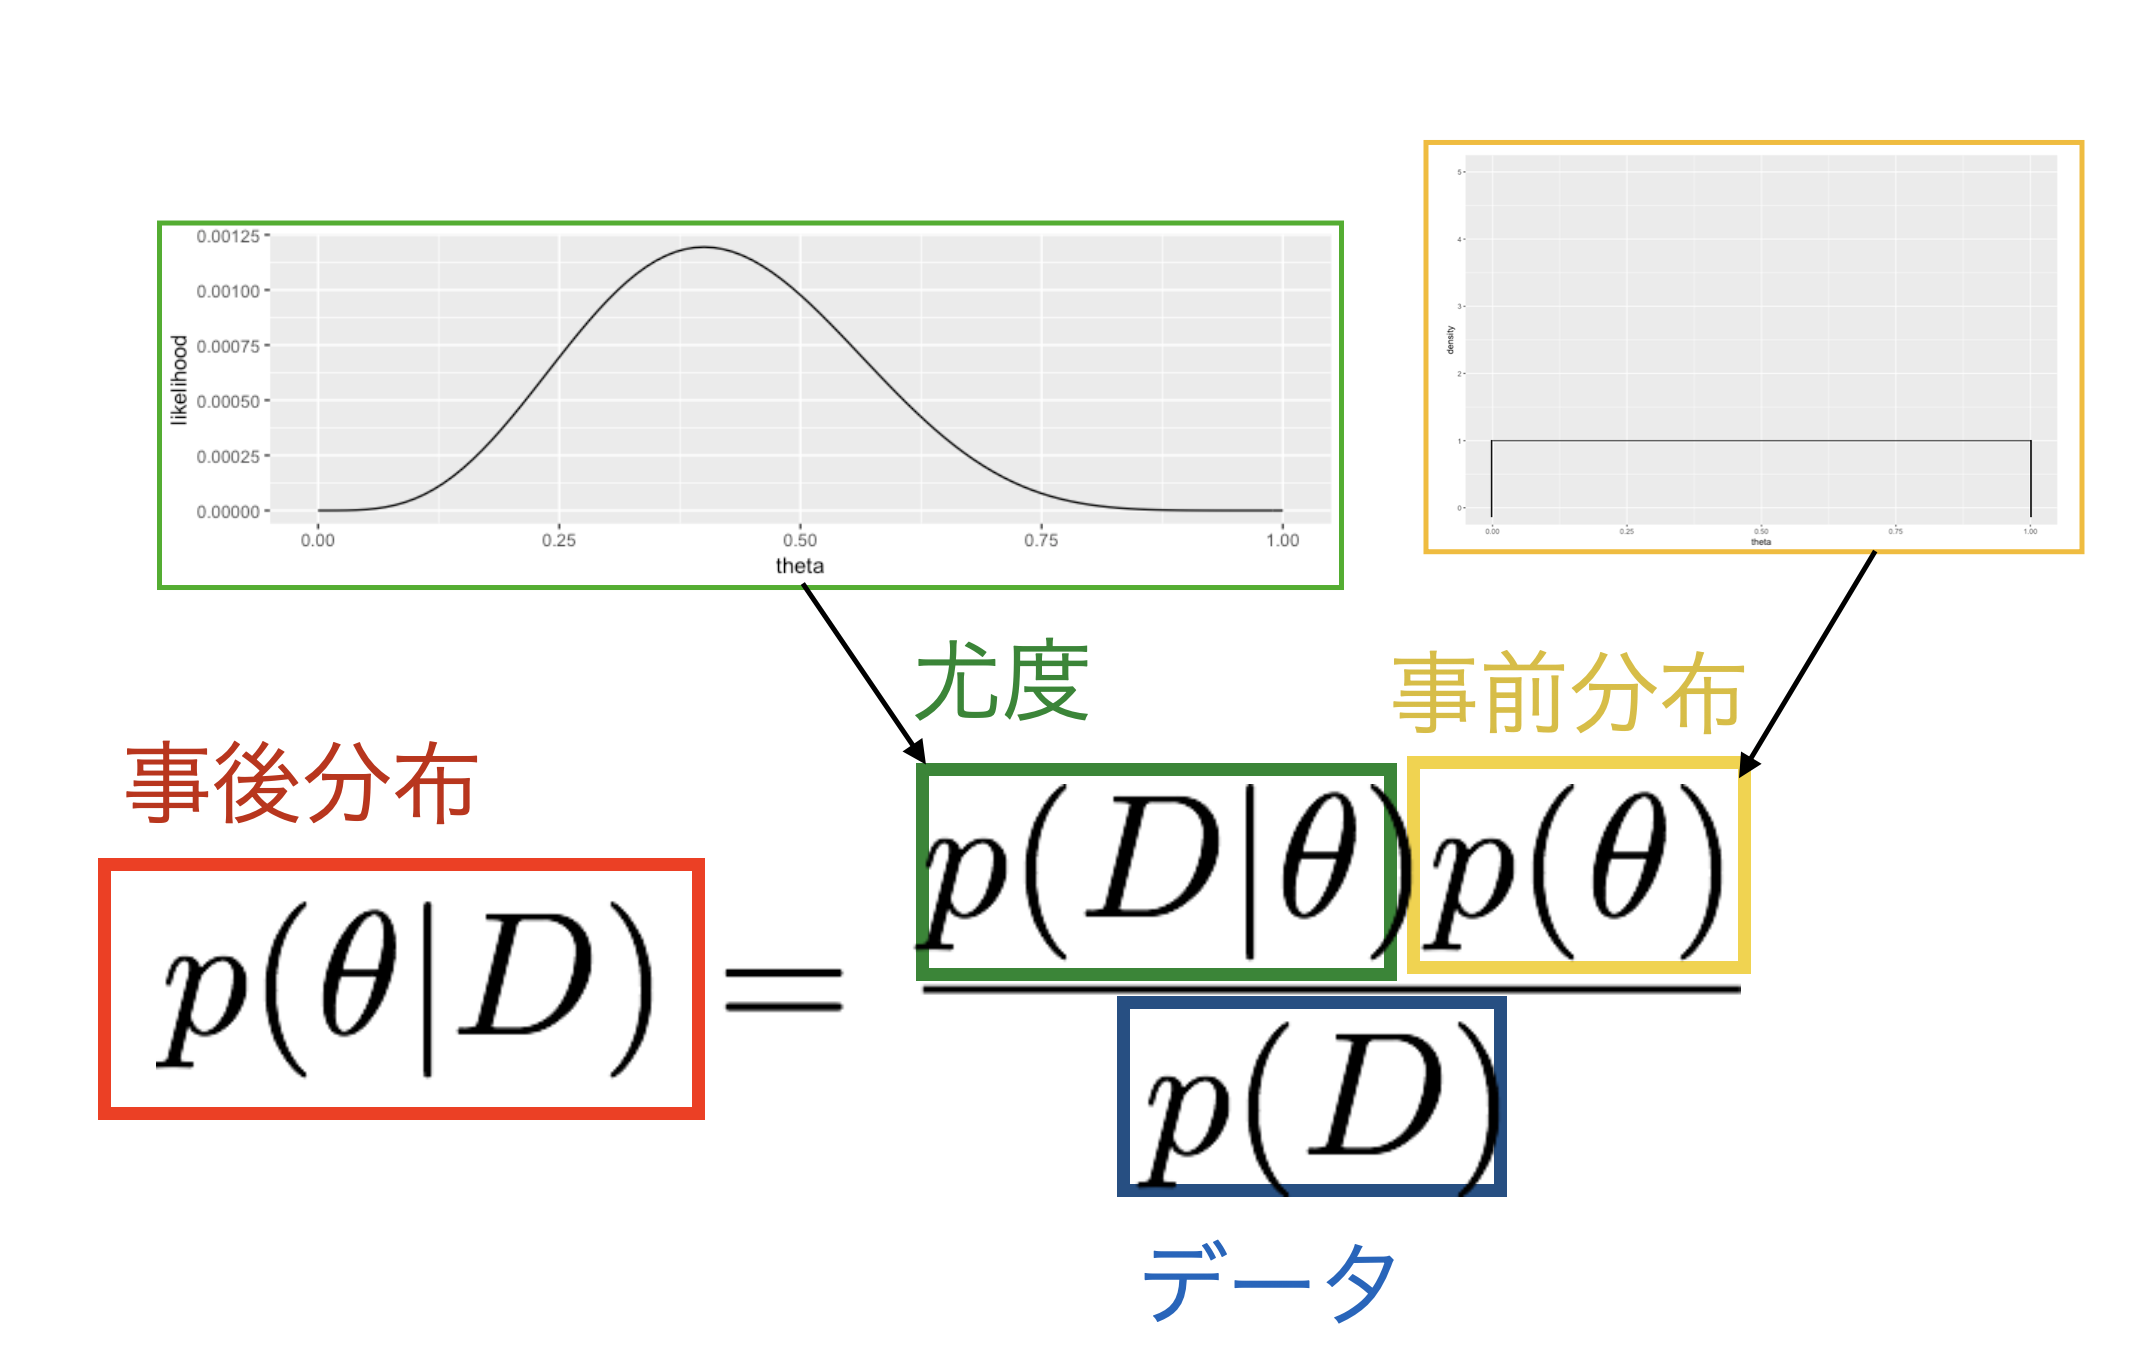
\includegraphics[keepaspectratio,width=12cm]{../images/text25/slide25_02.png}
    \caption{ベイズ推定の実際}
    \label{fig::25_02}
\end{figure}

分子が確率と確率の掛け算になっているので，イメージしにくいかもしれません。私個人のイメージでは，波の衝突のような感じだと思っています。X軸に沿って細かく数字を切り出して，逐一掛け合わせていくような方法のイメージでも良いかもしれません(図\ref{fig::25_03})。ちなみに事前分布が今回，無情報な一様分布ですので，尤度と組み合わせたところ，その高さは変わりますが形Shapeは変化しません。このように，事前分布を一様分布にしておくと，データと確率分布の関係，尤度の形をそのまま結果に反映させることができることになります。
\begin{figure}[ht]
    \centering
    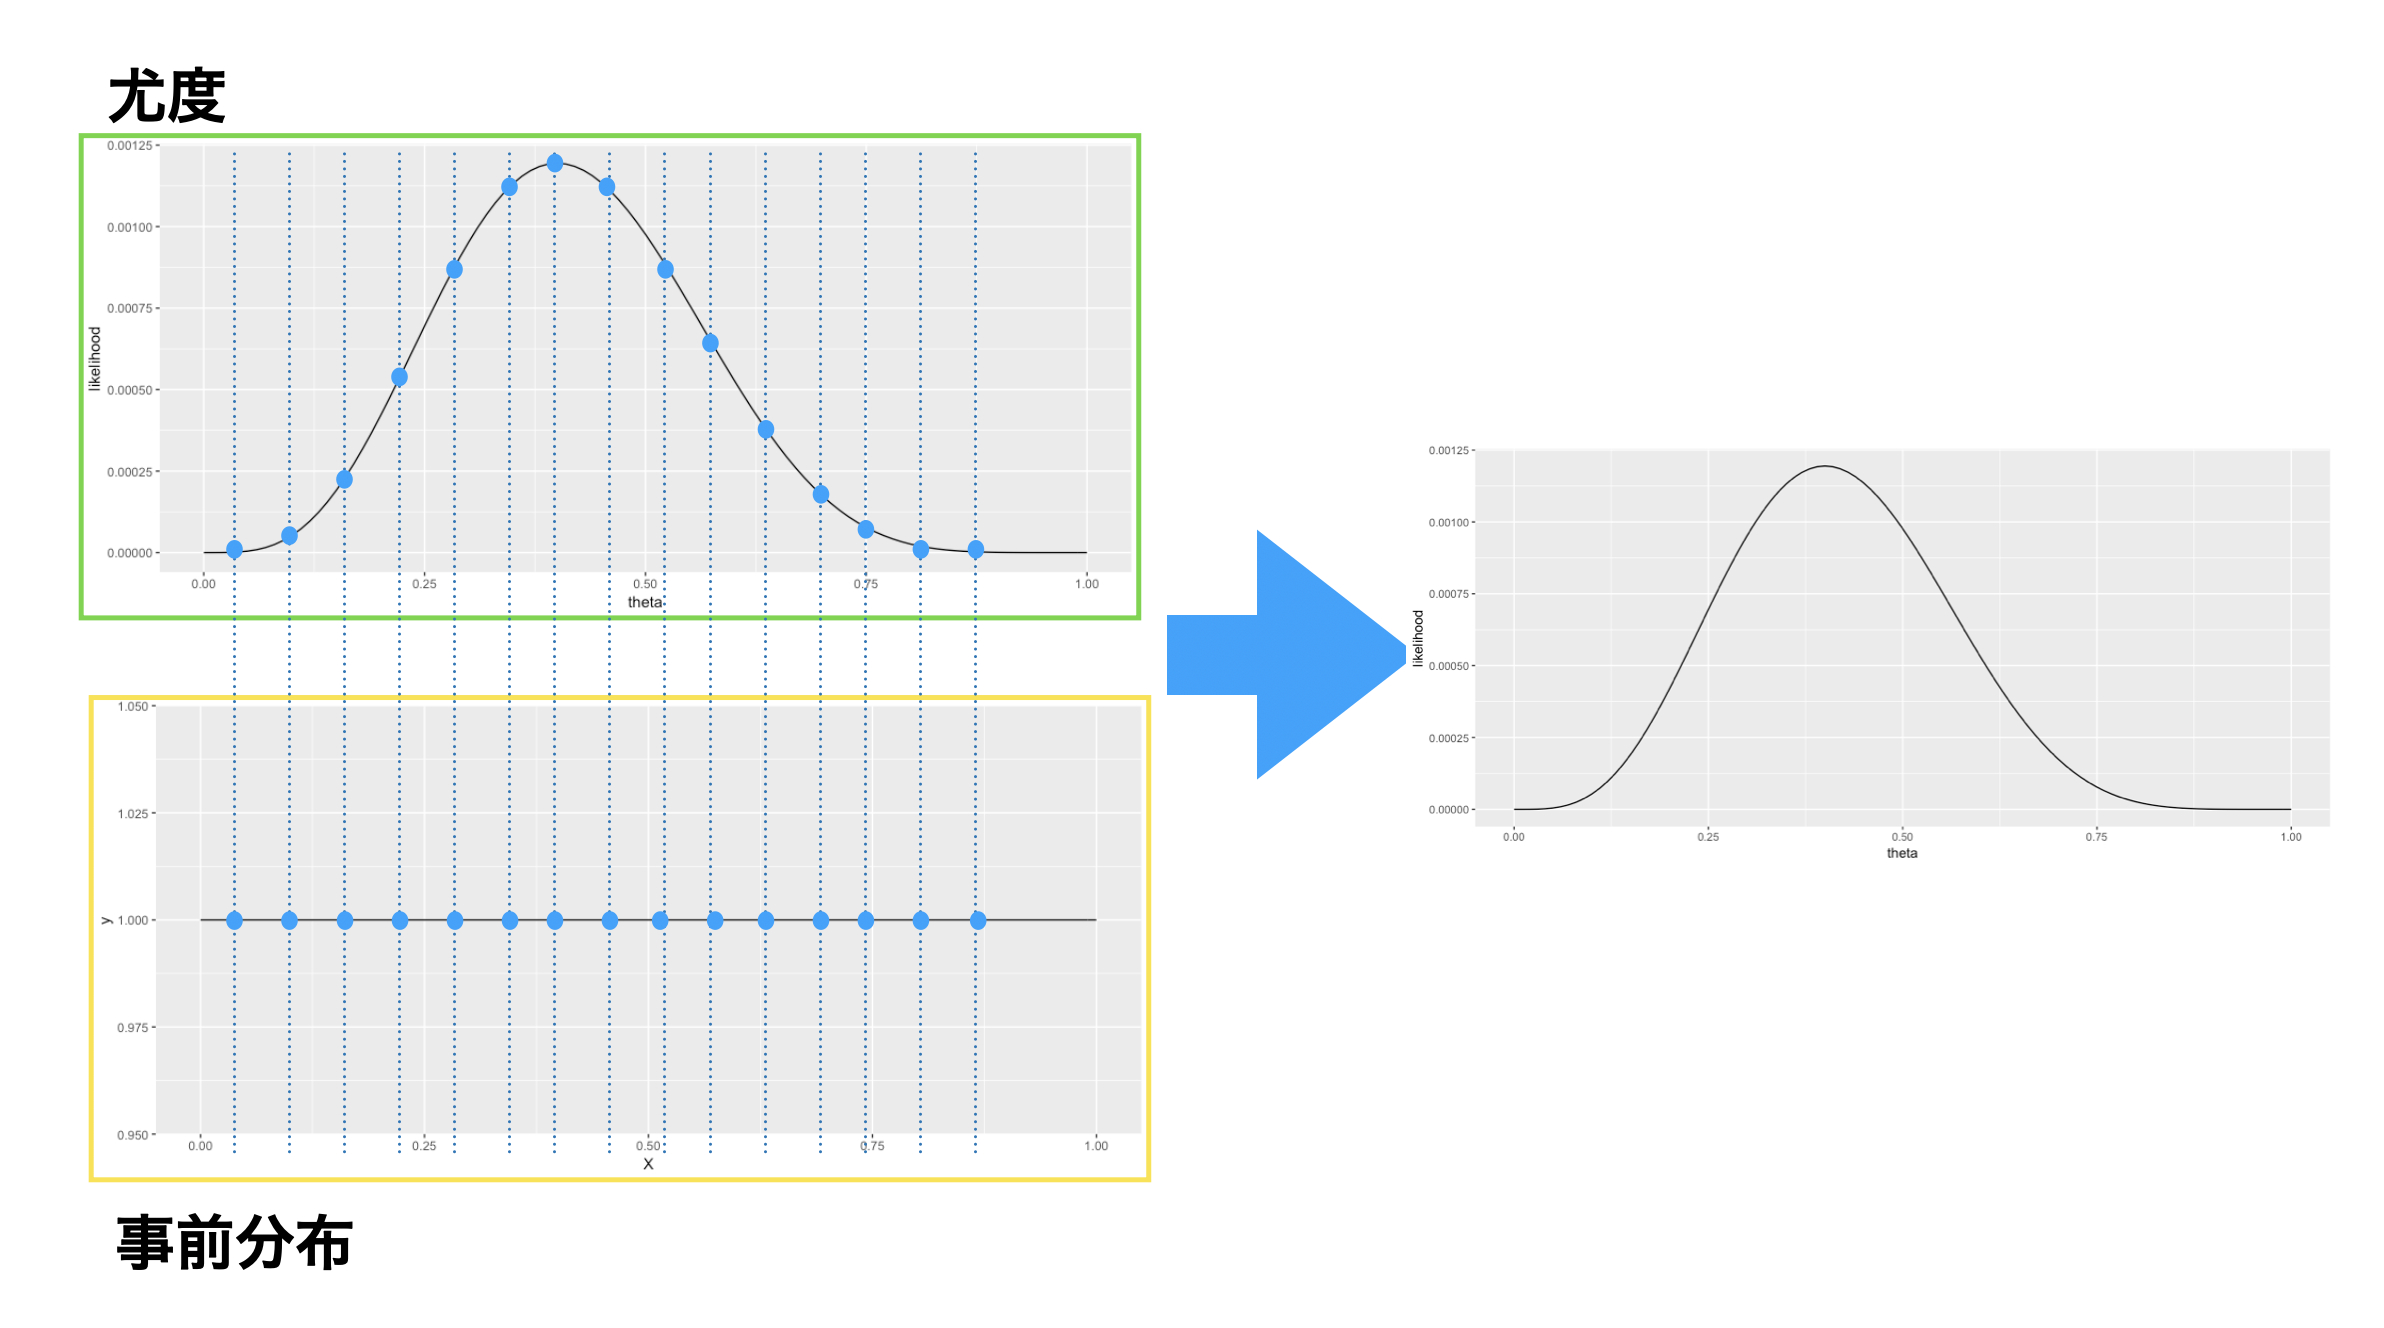
\includegraphics[keepaspectratio,width=12cm]{../images/text25/slide25_03.png}
    \caption{確率同士の掛け合わせ}
    \label{fig::25_03}
\end{figure}
さて，この掛け合わせた結果を$P(D)$，つまりデータの確率で割らないといけないのですが，ここは無視してしまいましょう。というのも，この分母が何をやっているかを考えれば，パラメータのような変わる数(変数)が含まれていないのでここは「定数」になっていることがわかります。分子のところは尤度と事前分布を掛け合わせたものですから，数字はすごく小さいのものになっているのでしょうが，最終的に左辺は事後分布という名の確率分布です。つまり，左辺は面積が1.0に規格化されており，分母は面積を1.0にするための，割り算用の定数に過ぎないということがわかります。我々はパラメータがどのあたりにあるのかが知りたいのですが，「ここにありそう」というのはそこの確率が高そうだ，ということであって，形さえわかれば縦軸の単位は別に詳しくわからなくても，横軸の位置を推測するのに苦労はない訳です。そういうわけで，分母は無視しちゃいましょう\footnote{繰り返しになりますが，実は深くベイズ推論を進めていくとこの分母というのが結構おもしろいもので，このモデルの中でデータがどれぐらい出てきそうなのか，というモデルとデータの適合度を測る目安に使えちゃうのです。がそれはまたの講釈で。}。この「形がわかればいい」というのを数学的に表すと，
\[ P(\mbox{事後分布}) \propto \mbox{尤度}\times \mbox{事前分布}\]
となります。$\propto$というのは，相似形である，という意味です。

さて，図\ref{fig::25_04}にあるように，事後分布が計算できました。これが$\theta$の推定結果ということになります。
\begin{figure}[ht]
    \centering
    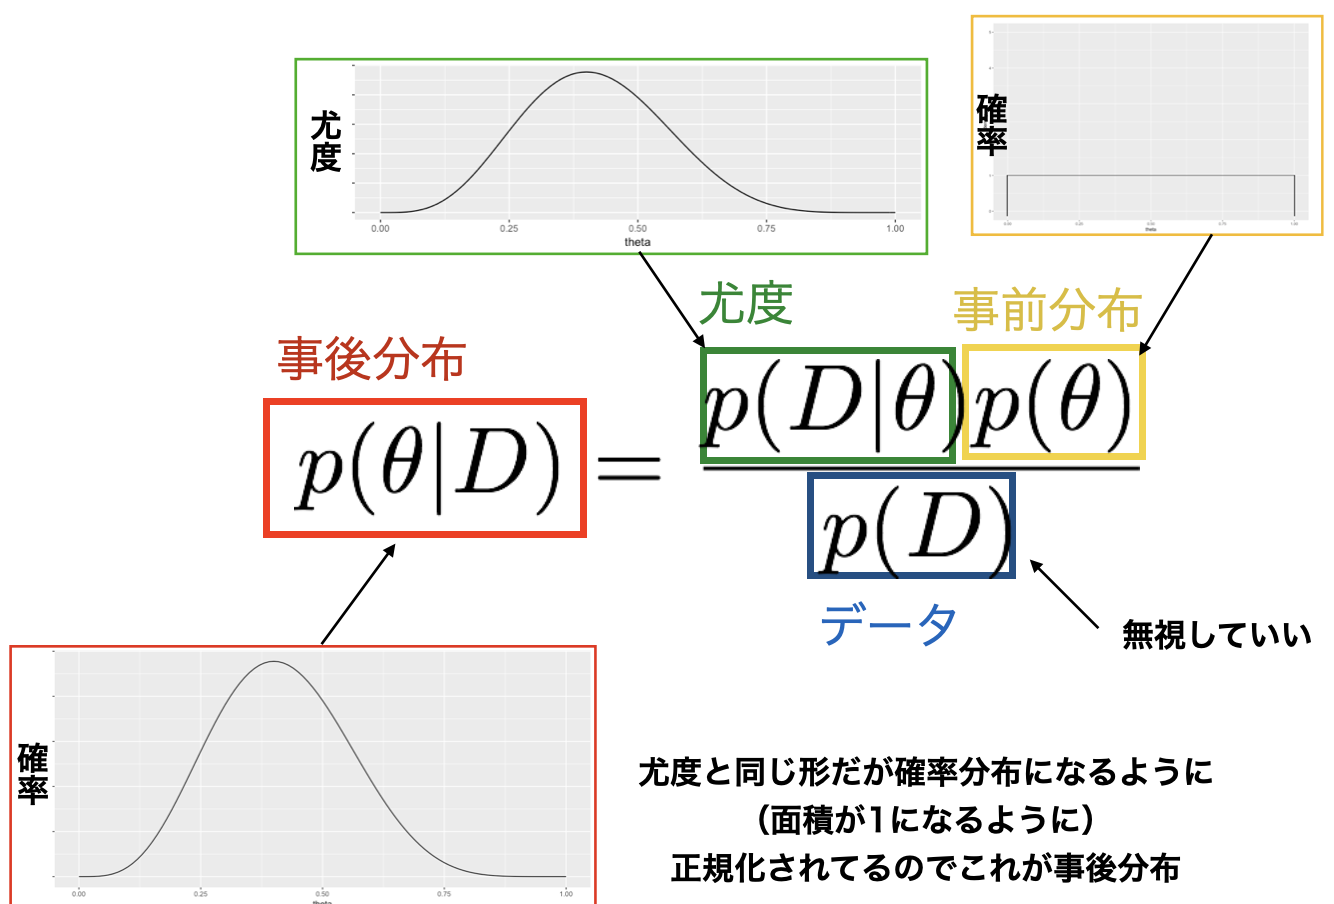
\includegraphics[keepaspectratio,width=12cm]{../images/text25/slide25_04.png}
    \caption{事後分布が計算できました}
    \label{fig::25_04}
\end{figure}

これで事後分布が計算できました。


心理学においても，実験者・研究者の無自覚的な影響が被験者に出ることなどを厳に慎むべし！という方法論的教えがありますから，事前分布に忌避感を持つ人がいるかもしれません。
% \item[事前分布と事後分布]ここまで事前・事後確率と呼んでいたものは，連続的な分布関数出会っても同様に機能する。計算方法として，確率の和が積分になることは，確率質量関数から確率密度関数に変わった時と同じである。また統計モデルにおいてベイズ推定を行う場合，何が更新されるのかイメージが掴みにくいことがある。我々が知りたかったことはパラメータの値であり，これについて割り当てられた確率がモデルによって更新されることを確認する。
% \begin{flushright}
%     $\to$ \citet{Maeda2017}18-23.や，\citet{豊田201606}のP.18--21
% \end{flushright}

% \item[尤度] ベイズの定理の分子における，尤度を今一度改めて確認する。特に回帰分析や，要因計画法における尤度関数を考え，どこに事前分布を置き事後分布を得るのかを，改めて確認しておくことが重要である。
% \begin{flushright}
%     $\to$ \citet{豊田201606}P.17--18や，\citet{kosugi2018}のP.117--122.
% \end{flushright}

% \item[周辺尤度]ベイズの定理の分母は周辺尤度と呼ばれる。今一度離散変数の例に戻って，周辺尤度の計算方法を考え，翻って連続変数の場合はどのようにして周辺尤度が計算されるかを理解する。この場合は積分の計算が重ねて行われることになるから，近年の技術的なブレイクスルーを見るまではベイズ推測がうまく扱えなかったという経緯がある。
% \begin{flushright}
%     $\to$ \citet{馬場201907}のP.54
% \end{flushright}

% \item[MCMC法]マルコフチェイン・モンテカルロ法は，困難であったベイズ推測を可能にした技術的ブレイクスルーであった。基本的なアイデアは，確率分布の形状を求める際に乱数を使って近似するということである。単純な乱数を用いた例から，之による確率分布の近似と積分計算の簡略化ができることを理解し，事後分布の相対的な形状近似ができるようになったことを学ぶ。
% \begin{flushright}
%     $\to$ \citet{Maeda2017}の7章，\citet{馬場201907}P.62--76
% \end{flushright}



\section{課題}
\paragraph{事後確率の計算}ある疾病は人口の0.05\%が罹患していることが分かっています。この病気の検査をしたとき，罹患している人が陽性になる確率は70\%です。また，罹患していない人が陽性となる確率は，0.1\%です。このとき，この検査で陽性と判定された人が，この病気に罹患している確率を求めなさい。

\end{document}
